%%%%%%%%%%%%%%%%%%%%%%% file template.tex %%%%%%%%%%%%%%%%%%%%%%%%%
%
% This is a general template file for the LaTeX package SVJour3
% for Springer journals.          Springer Heidelberg 2010/09/16
%
% Copy it to a new file with a new name and use it as the basis
% for your article. Delete % signs as needed.
%
% This template includes a few options for different layouts and
% content for various journals. Please consult a previous issue of
% your journal as needed.
%
%%%%%%%%%%%%%%%%%%%%%%%%%%%%%%%%%%%%%%%%%%%%%%%%%%%%%%%%%%%%%%%%%%%
%
% First comes an example EPS file -- just ignore it and
% proceed on the \documentclass line
% your LaTeX will extract the file if required
\begin{filecontents*}{example.eps}
%!PS-Adobe-3.0 EPSF-3.0
%%BoundingBox: 19 19 221 221
%%CreationDate: Mon Sep 29 1997
%%Creator: programmed by hand (JK)
%%EndComments
gsave
newpath
  20 20 moveto
  20 220 lineto
  220 220 lineto
  220 20 lineto
closepath
2 setlinewidth
gsave
  .4 setgray fill
grestore
stroke
grestore
\end{filecontents*}
%
\RequirePackage{fix-cm}
%
%\documentclass{svjour3}                     % onecolumn (standard format)
%\documentclass[smallcondensed]{svjour3}     % onecolumn (ditto)
%\documentclass[smallextended]{svjour3}       % onecolumn (second format)
\documentclass[smallextended,twocolumn]{svjour3}          % twocolumn
%
\journalname{Behavior Research Methods}
\smartqed  % flush right qed marks, e.g. at end of proof
%
\usepackage{graphicx}
%
%usepackage{mathptmx}      % use Times fonts if available on your TeX system
%
\usepackage[natbibapa]{apacite}

%\usepackage{tabularx}
\usepackage{amsmath}
\usepackage{booktabs}
\usepackage{units}
\usepackage[draft]{hyperref} %tmp added draft option for spilling refs
\usepackage{wrapfig}
\usepackage{todonotes}
\newcommand{\eg}{e.g., }
\newcommand{\remodnav}{REMoDNaV}

\begin{document}

\onecolumn
\title{REMoDNaV: Robust Eye Movement Detection for Natural Viewing } %\\ (remodnav)
%\titlenote{The title should be detailed enough for someone to know whether the article would be of interest to them, but also concise. Please ensure the broadness and claims within the title are appropriate to the content of the article itself.}
\author{%
  Asim~H.~Dar \and
  Adina~Wagner \and
  Ulrike~Schnaithmann \and
  Isabel~Dombrowe \and
  Michael~Hanke}

\institute{F. Author \at
              first address \\
              Tel.: +123-45-678910\\
              Fax: +123-45-678910\\
              \email{fauthor@example.com}           %  \\
%             \emph{Present address:} of F. Author  %  if needed
           \and
           S. Author \at
              second address
}


%\affil[1]{Psychoinformatics Lab, Institute of Psychology, Otto-von-Guericke University, Magdeburg, Germany}
%\affil[2]{Department of Cognitive Psychology: Judgment, Decision Making, Action, Fern Universität, Hagen,
%Germany} %TODO: Correct?
%\affil[3]{Center for Behavioral Brain Sciences, Magdeburg, Germany}

\date{Received: date / Accepted: date}

\maketitle

%Please list all authors that played a significant role in the research involved in the article. Please provide full affiliation information (including full institutional address, ZIP code and e-mail address) for all authors, and identify who is/are the corresponding author(s).

\begin{abstract}

%Abstracts should be up to 300 words and provide a succinct summary of the article. Although the abstract should explain why the article might be interesting, care should be taken not to inappropriately over-emphasize the importance of the work described in the article. Citations should not be used in the abstract, and the use of abbreviations should be minimized. If you are writing a Research or Systematic Review article, please structure your abstract into Background, Methods, Results, and Conclusions.
Tracking of eye movements during cognitive tasks is an established metric for many types of experimental paradigms in both psychology and cognitive neuroscience. In such experiments, the usage of more complex and lengthier visual stimuli has made algorithmic approaches --- in detecting eye movement events as saccades and fixations --- the most pragmatic option. A recent analysis has revealed that current algorithms for detecting eye movements are lackluster when it comes to processing eye tracking data from subjects viewing dynamic stimuli such as video sequences. We aimed to design an algorithm that has comparable performance to currently used software of the same purpose but also specially tuned to detect different events in data from dynamic stimuli. We compared the output of our algorithm to a data set which had manually annotated events to compare performance with human viewers --- which we consider as the gold standard when it comes to accuracy. In addition, we compared our algorithm to a currently developed one to see if the performance is up to par. After validating its functionality, we applied our algorithm to noisy eye tracking data to see how if the results were biologically feasible. We found that our algorithm performs relatively well and particularly stands out when it comes to the evaluation of data from dynamic stimuli. To establish broad distribution and applicability we provided the option to include individual parameters based on the paradigm and equipment used by the investigator and bundled it into an open-source and well documented repository.



\keywords{%
eye tracking \and
adaptive detection algorithm \and
saccade detection algorithm \and
statistical saccade analysis \and
glissade detection \and
adaptive threshold algorithm \and
data preprocessing
}
\end{abstract}

%\todo[inline]{The scope of the article is a "Data Note" that describes new "derived" data generated from the raw eyetracking data released by the studyforrest project. I propose to produce two types of artifacts: 1. filtered/preprocessed eyetracking data, and 2. a list with detected saccades for each recording.}

%\todo[inline]{It would be good to also release fully preprocessed data. Apart from applying the chosen filter, it would also make sense to me to temporally down-sample the data. What would be a practical sampling rate that reduces the data size (and some noise), but does not negatively impact most potential analyses? 100 Hz? 200 Hz? Even in the latter case it would still be a 5x reduction in size.}
%\todo[inline, backgroundcolor = green]{250 Hz is the lower limit to detect most saccades (Kern 2000). However,the downsampled data did not reach the same accuracy level as the higher frequency data, probably because the algorithm was designed to work on higher frequencies (as stated by the authors). Therefore we left it at the 1000 Hz frequency}

\twocolumn
\section*{Introduction}\label{intro}

%\todo[inline]{\textit{make connection to studyforrest. studyforrest has eyetracking data. why is it necessary to have that preprocessed?}}

% The data used for this thesis originates from the open science project 'studyforrest'. It centers around two large data acquisition phases employing the movie 'Forrest Gump' as stimulus. \cite{Hanke.2014,Hanke.2016} The project provides a large variety of collections of data to enable fellow researchers to build upon existing knowledge and further extend the dataset. Along other measures, the eye gaze coordinates were being recorded during the original sessions. Contrarily to the standard automatic detection process we applied an adaptive algorithm to the eye movement data to provide a more precise computation of saccades and fixations. 

A spreading theme in cognitive neuroscience is the usage of dynamic and natural stimuli as opposed to isolated and distinct imagery used in classical studies. Using such stimuli we are able to observe the nuances of cognition in a more natural environment. Some interesting applications include the determination of neural response to changes in facial expression \citep{Harris2014}, understanding complex social interactions by using videos \citep{Tikka2012} and more untouched themes such as the underlying processing of music \citep{Toiviainen2014}. \todo{"Quantify the amount of correlation between response and stimuli"?} In these studies, a physical measurement is needed to quantify the amount of correlation between response and stimuli. One measure that is useful and well established for such use cases is data obtained from eye tracking. Eye tracking is a flexible measurement which has proven its worth in a variety of studies ranging from the understanding of visual attention \citep{HantaoLiu2011}, memory \citep{Hannula2010} and language comprehension \citep{Gordon2006}. The raw eye tracking data provided by eye tracking devices however is rarely used "as is". Instead, in order to disentangle different cognitive, oculomotor, or perceptive states associated with different types of eye movements, most research relies on a classification of eye gaze data into distinct eye movements categories (TODO: this needs a citation). \\
Our interest is the usage of eye gaze data as obtained from eye tracking from the studyforrest dataset--- a dataset containing a variety of outputs from subjects viewing natural and dynamic stimuli in the form of a full length movie \citep{Hanke2016}. The available eye gaze data in this dataset stems from a high-quality laboratory recording, but also from simultaneous eye-tracking and functional magnetic resonance imaging (fMRI) acquisition in the bore of an MRI scanner with higher spatial uncertainty and noise level. In order to effectively use this eye gaze data, we searched for an algorithm that would help us sort out different eye related events, namely, saccades, fixations, and post-saccadic oscillations \todo{and smooth pursuit?}. As advocates of open-source software and scientific reproducibility we focused on non-commercial algorithms that were both well documented (published works) and freely available. Conveniently, a recent study \citep{Andersson2017} took on the task of evaluating eye gaze data algorithms on different sets of stimuli and compared them to human "coders" --- which were human participants who marked events in eye gaze data on a GUI. While the algorithms worked well for static stimuli, to our disappointment, the authors concluded that none of the algorithms performed remarkably well when it came to dynamic stimuli. The analysis of eye gaze during dynamic stimulation however can lead to a deeper understanding of behavioral or cognitive processes and is relevant for a multitude of fields, from cinematography, to industrial engineering and human-computer interactions, marketing, or our own field, computational neuroscience \citep{Duchowski2002}. \\
One of the most successful algorithms capable of classifying saccades, fixations, and post-saccadic oscillation as evaluated by \citet{Andersson2017} was an adaptive, velocity-based algorithm proposed by \citet{Nystrom2010AnData}. Even though the algorithm performed poorly on dynamic stimuli, its classification performance was good for static stimulation. The algorithm, henceforth referred to as \textit{NH}, detects fixations, saccades, and post-saccadic oscillations (termed "glissades"), and determines the velocity threshold used in classification based on the data's noise level. We initially tried to apply the NH algorithm with no modifications to our eye gaze data. This however yielded implausible results. For example, the average and median durations of eye movements classed as fixations exceeded durations reported in the literature \citep{holmqvist2011eye}; \citep{dorr2010variability}\todo{fix this type of citation. in my own templates, I use npcite for this} by up to factor 2. Additionally, especially for noisy data, the NH algorithm classified too few fixations, as remarked previously by \citet{Friedman2018} already, because it discarded potential fixation events that contained artifacts such as blinks. Consequently, the NH algorithm was unsuitable for our noisy, but precious data. Therefore, based on our use case in the studyforrest dataset, we set out to extend and enhance the algorithm for use with --- potentially noisy --- data from dynamic stimulation. For this, we identified a number of areas that needed to be improved. For one, dynamic stimuli evoke smooth pursuit movements, slow motions of the eye as it follows a moving target. If this type of eye movement is not properly detected, this will introduce erroneous fixation and saccade events (which smooth pursuits would be classified into instead). \todo[inline]{identify a number of areas we wanted to improve: smooth pursuit detection; do something with the artifacts (recall what exactly...), check a few old github issues for more insights...}


The aim of this article is to describe a novel, data-driven algorithm that is based on and extends
the NH algorithm to yield robust results for dynamic stimulation. For this... \todo[inline]{outline briefly what our algorithms does that is missing so far}
In order to facilitate its usage and to remove barriers in software retrieval, the resulting algorithm is packaged in an accessible and open-source Python module REMoDNaV.\\
\todo{add sth about documentation} REMoDNaV contains two main novelties: For one, because dynamic stimulation contains moving visual targets, it detects \textit{smooth pursuits}. Contemporary algorithms rarely provide this functionality (see e.g. \cite{LARSSON2015145}\todo{interesting inability for umlaute }; \cite{Komogortsev2013} as existing algorithms with smooth pursuit detection, though)\\
\todo{list smooth pursuit detecting algorithms and find out whether they have deficiencies for dynamic stimuli} In order to evaluate REMoDNaVs classification performance, we compare its output to the original algorithm by \citet{Nystrom2010AnData} and manual human annotation of eye movements. Secondly, as our primary use case stems from noisy data obtained from natural viewing, the algorithm is created specifically to compute robust results even for low-quality data. We demonstrate this by comparing algorithm performance on data with different qualities, but from the same underlying stimulation.



\todo{add advantages with regard to parameter selection: few subjective settings as in NH, intelligent internal decisions based on data characteristics}


%TODO:Elaborate to include different approaches that current algorithms took use?

\todo[inline]{One outcome of Andersons algorithm comparison was that (I quote the abstract): " The main conclusion is that current detectors of only fixations and saccades work reasonably well for static stimuli, but barely better than chance for dynamic stimuli." This is a good starting point for us.}
\todo[inline]{Our reasoning is that we want an algorithm to work with dynamic stimuli. We should elaborate on why this requires capabilities to include smooth pursuits, and then say that contemporary algorithms rarely have this capability}


\section*{Methods}\label{methods}
%Methods (3 sections; our algo, comparison to current algos, application on studyforrest dataset)


\subsection*{Implementation}\label{impl}
 
%\todo[inline]{\textit{Elaborate on how the algorithm works;For software tool papers, this section should address how the tool works and any relevant technical details required for implementation of the tool by other developers.}}

The algorithm functions in two major steps: firstly, eye tracking data is preprocessed by applying relevent filters, calculating velocity and acceleration of movements. In the second stage, events are detected with the final outputs being labeled as saccades, fixations, post-saccadic oscillations (PSOs) or smooth pursuit.
\begin{enumerate}
\item{Preprocessing}

 To prevent extreme changes in eye tracking data, a spike filter is applied (TODO: Which one is this exactly? Cite) followed by the calculation of velocity of eye movements based on the co-ordinate data,  dimensions of the screen, distance of the participant from the screen and the sample rate of the eye tracker. A configurable maximum velocity is enforced, with calculated values above this level being replaced by this set value. Using these velocities, acceleration of the eye movements is computed. 
 At this stage, a variety of optional functionality is also available. On demand, the algorithm can: 
 \begin{enumerate}
 	\item Mask data around signal loss (such as eyeblinks)
 	\item Apply Savitzy-Golay filter (for noise reduction) 
 	\item Compute additional movement velocities after additional medial filtering
 	
 \end{enumerate}

\item{Event detection}
\begin{enumerate}

 \item The entire time series is chunked into intervals between major saccades to be able to accommodate data without a short trial structure. Major saccades are located by thresholding the \textit{median-}filtered velocities with a critical velocity value. This value is determined by the entire input data, following the same steps as the algorithm designed by \citet{Nystrom2010AnData}. Continuing in the same vein, for each saccade window (sorted by the total magnitude of its velocity), saccade onset and offset is detected as well as PSOs --- using the by \citet{Nystrom2010AnData} --- but instead using on/offset thresholds that are determined in the temporal vicinity around a respective candidate window. By default, this  is from one second before to one second after the window boundaries.
 
 Additionally, saccadic detection is terminated earlier if a maximum saccade frequency across the entire input data is reached--- this value is configurable and by default is set to \unit[2]{Hz}
 
 \item In a locally adaptive manner, events are then detected \textit{between} the major saccades detected earlier. This is carried out by firstly further subdividing these intervals into segments without any missing data. Using a velocity threshold --- determined from the specific time window only --- saccade detection follows if its duration exceeds the minimum saccade length and is within a certain minimum distance from neighboring saccades (default: \unit[130]{ms}). 
 The remaining unlabeled time window that is longer than a configured minimum duration (default: \unit[40]{ms}), velocities are recomputed after low-pass filtering (default cutoff: \unit[4]{Hz}) and segments exceeding a maximum fixation velocity threshold are labeled as smooth pursuits, while everything else as fixations. Pursuit on/offset employs the same algorithm as \citet{Nystrom2010AnData} used for determining saccade on/offset, but with a configurable, fixed velocity threshold (default: \unit[2]{deg/s}). 
   
\end{enumerate}
\end{enumerate}

%% start with a plain list, later work into flow chart or table...
% Adina: commenting that out for now
%\begin{enumerate}
%  \item Preprocessing
%    \begin{enumerate}
%      \item Apply spike filter (cite)
%      \item (opt) Mask data around signal loss
%      \item (opt) Apply Savitzy-Golay filter for noise reduction
%      \item Compute movement velocities
%      \item Impose configurable maximum velocity (replace exceeding values with previous estimate)
%      \item Compute movement accelaration from velocity estimates
%      \item (opt) Compute additional movement velocities after additional (heavy) median filtering
%
%    \end{enumerate}
%  \item Event detection
%    \begin{enumerate}
%      \item Time series chunking into interval between \textit{major} saccades, to be able to accommodate data without a (short) trial structure
%        % objective 1: chunk the timeseries into meaningful segments, data might not have
%        % a trial structure
%        \begin{enumerate}
%          \item Determine location of major saccades by thresholding the \textit{median-}filtered velocities with a critical velocity value determined from the entire input data following an algorithm by \citep{Nystrom2010AnData}
%          \item For each saccade candidate window (sorted by total velocity magnitude, largest first), perform saccade onset and offset detection (incl. PSO detection) via the \cite{Nystrom2010AnData} algorithm, but using velocity on/offset thresholds that are determined in the temporal vicinity around a respective candidate window (by default from \unit[1]{s} before to \unit[1]{s} after the window boundaries).
%          \item Saccade detection is terminated early, if a configurable maximum saccade
%            frequency across the entire input data is reached (default: \unit[2]{Hz})
%        \end{enumerate}
%    % outcome: inter-saccade-intervals of >~500ms length (like trials)
%      \item Locally adaptive detection of eyemovement events with each intervall between
%        previously detected major saccades
%        \begin{enumerate}
%          \item Further subdivide the interval into windows without missing data
%          \item Within each window, perform saccade detection, if its duration exceeds
%            a minimum-length saccade with minimum distance to neighboring saccades
%            (default: \unit[130]{ms}), using velocity thresholds determined from the
%            specific time window only
%          \item For each remaining unlabeled time window that is longer than a
%            configured minimum duration (default: \unit[40]{ms}), re-compute velocities
%            after low-pass filtering (default cutoff: \unit[4]{Hz}), label segments
%            exceeding a maximum fixation velocity threshold
%            as smooth pursuit, and everything else as a fixation. Pursuit on/offset
%            detection employs the same algorithm from \cite{Nystrom2010AnData} used for
%            determining saccade on/offset, but with a configurable, fixed velocity threshold
%            (default: \unit[2]{deg/s})
%        \end{enumerate}
%
%    \end{enumerate}
%\end{enumerate}

\todo[inline]{possibly have figure on the algorithm concept and general approach}
\todo{test}

\begin{table*}[t]
\caption{Algorithm parameters and their default values
\todo[inline]{recall citation for choosing value of max\_initial\_saccade\_freq, pursuit\_velthresh}}
\label{tab:parameters}
\small
\begin{tabular}{lp{85mm}l}
\textbf{Name} & \textbf{Description} & \textbf{Value} \\
 & & \\
\multicolumn{3}{l}{\textit{Preprocessing (in order of application during processing)}} \\
\texttt{px2deg} &
size of a single (square) pixel in degrees of visual angle &
no default [\unit{deg/s}]\\
\texttt{sampling\_rate} &
temporal data sampling rate/frequency &
no default [\unit{Hz}]\\
\texttt{min\_blink\_duration} &
missing data windows shorter than this duration will not be considered for \texttt{dilate\_nan}&
\unit[0.02]{s}\\
\texttt{dilate\_nan} &
duration for which to replace data by missing data markers on either side of a
signal-loss window &
\unit[0.01]{s}\\
\texttt{median\_filter\_length} &
smoothing median-filter size (for initial data chunking only) &
\unit[0.05]{s}\\
\texttt{savgol\_length} &
size of Savitzky-Golay filter for noise reduction&
\unit[0.019]{s}\\
\texttt{savgol\_polyord} &
polynomial order of Savitzky-Golay filter for noise reduction&
2\\
\texttt{max\_vel} &
maximum velocity threshold, will issue warning if exceeded to inform about
potentially inappropriate filter settings&
\unit[1000]{deg/s}\\

\\\multicolumn{3}{l}{\textit{Event detection}} \\
\texttt{min\_saccade\_duration} &
minimum duration of a saccade event candidate &
\unit[0.01]{s}\\
\texttt{max\_pso\_duration} &
minimum duration of a post-saccadic oscillation (glissade) candidate &
\unit[0.04]{s}\\
\texttt{min\_fixation\_duration} &
minimum duration of a fixation event candidate &
\unit[0.04]{s}\\
\texttt{min\_pursuit\_duration} &
minimum duration of a pursuit event candidate &
\unit[0.04]{s}\\
\texttt{min\_intersaccade\_duration} &
no saccade detection is performed in windows shorter than twice this value, plus minimum saccade and PSO duration&
\unit[0.04]{s}\\
\texttt{noise\_factor} &
adaptive saccade onset threshold velocity is the median absolute deviation of velocities in the window of interest, times this factor (peak velocity threshold is twice the onset velocity); increase for noisy data to reduce false positives \citep[equivalent: 3.0]{Nystrom2010AnData}&
5\\
\texttt{velthresh\_startvelocity} &
start value for adaptive velocity threshold algorithm \citep{Nystrom2010AnData}, should
be larger than any conceivable minimum saccade velocity &
\unit[300]{deg/s}\\
\texttt{max\_initial\_saccade\_freq} &
maximum saccade frequency for initial detection of major saccades, initial data
chunking is stopped if this frequency is reached (should be smaller than an expected
(natural) saccade frequency in a particular context)&
\unit[2]{Hz}\\
\texttt{saccade\_context\_window\_length} &
size of a window centered on any velocity peak for adaptive determination of
saccade velocity thresholds (for initial data chunking only) &
\unit[1]{s}\\
\texttt{lowpass\_cutoff\_freq} &
cut-off frequency of a Butterworth low-pass filter applied to determine drift
velocities in a pursuit event candidate &
\unit[4]{Hz}\\
\texttt{pursuit\_velthresh} &
fixed drift velocity threshold to distinguish periods of pursuit from periods of fixation &
\unit[2]{deg/s}\\

\end{tabular}
\end{table*}


\todo[inline]{did we enforce a minimum saccade duration?}

%\subsection*{Going beyond basic dynamic stimuli; the studyforrest dataset}
%\todo[inline]{\textit{fix/update text below}}

%\todo[inline]{this sections describes the method that produces the
%data artifacts. what kind of filtering? What kind of saccade detection algorithm? It should contain an \textbf{ultra-brief} summary of the eyetracking details from \cite{HAK+16}, but otherwise just refer to this article for details.}

%In the original study, Hanke et. al \cite{Hanke.2016} split 30 participants into groups of 15 and placed one half in a fMRI scanner set-up and the other in a lab setting while recording eye movements during the two hour movie stimulus. For further technical details please refer to the original article. As part of an unpublished Bachelor project, we compared different filter and saccade detection algorithm combinations. To quantify the precision of the combination, the correlation between peak velocity and amplitude of all saccades, known as the main sequence, and the inherent $r^2$ values were computed. The higher the data fit to the assumed main sequence $MS$ curve $MS=mx^n$ the more precise the filter-algorithm option. The combination of Savitzky-Golay filter and an adaptive detection algorithm by Nyström and Holmqvist proved to be most precise and was used for further analysis. The respective algorithm employs a daten-driven threshold which automatically adjusts to local noise levels. It consists of five steps including filtering with Savitzgy-Golay, peak saccade detection, saccade on- and offset determination, as well as glissade and fixation identification. Parameters used for computation were kept exactly as suggested by the authors. According to the algorithm, after detecting saccades and follow-up glissades, the left over movements between saccades were considered fixations. Due to higher noise in dynamic stimuli and the longer recording period this assumption did not hold in the studyforrest dataset. Therefore, an additional velocity limit of 6.58 $\frac{\circ}{s}$ and amplitude of 2 $^\circ$ during a fixation was integrated as these values are commonly viewed as fixation thresholds.\cite{Holmqvist.2011,Henderson.1997}

%Methods should include a brief discussion of allowances made (if any) for controlling bias or unwanted sources of variability, and the limitations of the datasets.



%\todo[inline]{\textit{brief description of the nature and amount of data released, and in which format it is released in}}
%The data is divided into lab and scanner data and released as separate text files for each movie segment per participant. This results in a set of 240 .txt files. The first step of the detection process includes disregarding biologically implausible values and blinks followed up by  Savitzky-Golay filtering. The output files display the velocity, acceleration, point in time and pixel coordinates for each sample and are released separately to enable additional calculations. These files are then further processed to detect saccades, glissades and fixations. The final output includes the typical eye tracking information on each movement event: time and coordinates for on- and offset, amplitude, peak velocity and average velocity. (peak velocity was not calculated for fixations)  

\subsection*{Operation}\label{op}

\remodnav\ is free and open-source software, written in the Python language and
released under the terms of the MIT license. In addition to the Python standard
library it requires the Python packages
NumPy \citep{oliphant2006guide},
Matplotlib \citep{hunter2007matplotlib},
statsmodels \citep{seabold2010statsmodels},
and SciPy \citep{JOP+2001} as software dependencies.
Furthermore, DataLad \citep{HH+2013},
and Pandas \citep{mckinney2010data} have to be available for assessing
correct operation via the \remodnav\ test battery. \remodnav\ itself,
and all software dependencies are available on all major operating systems.
There are no particular hardware requirements for running the software
other than sufficient memory to load and process the data.



\section*{Validation analyses}\label{ana}

\todo[inline]{three major types of comparison: with andersson human labeling, stats of forrest lab recording with andersson video data stats, forrest lab vs forrest mri stats. the goal is to show that we are similar to humans, as good (or better) as other algorithms (by comparison with scores in andersson2017), and proceduce "similar" results on a different movie dataset, and similar results across two different qualities of recordings with the same stimulus (lab vs MRI). No more, no less IMHO. This all translates to three use cases: trial-by-trial data (from anderson), good movie data without trial structure (forrest lab), bad movie data (forrest mri)}

%THIS SECTION  WILL BASICALLY SHOW THE INPUTS AND THE OUTPUTS(RESULTS BASICALLY)
%\todo[inline]{\textit{Testing and comparison --- explaining rationale of the compared algorithms ie they were winners in the anderson paper}}
We applied our algorithm to two datasets, each to fulfill different objectives. First, in order to validate REMoDNaV, we used the dataset made available by \citep{Andersson2017} to see how our algorithm compared against the algorithm it is based on and manual human annotation of eye gaze events. This was done to be sure to not impair the existing NH algorithms performance, and to evaluate whether REMoDNaV actually improves eye movement detection during dynamic stimulation. Secondly, we used our algorithm on the studyforrest dataset \citep{Hanke2016} to see the results of dynamic stimuli under two different noise conditions: A high-quality dataset from a laboratory setting, and low-quality data from a simultaneous fMRI and eye gaze acquisition. This analysis was used to provide a demonstration of how robust the algorithm performs.

\subsection*{Evaluation of the algorithm: comparing outputs against human coders and a current algorithm}\label{ana_1}

The dataset provided by \citep{Andersson2017} consists of eye gaze data produced from viewing stimuli from three distinct categories --- images, moving dots and videos. In addition to the eye tracking metadata (eye tracker sampling rate, size of the screen raw eye gaze data, distance from screen) and eye gaze data (coordinates), each frame was also labeled by two human observers to assign the event they thought it was. A total of six different labels were used, namely, fixation, saccade, post-saccadic oscillation, smooth pursuit, blink and undefined (a sample that did not fit any other category). \\
To compare the REMoDNaV results to the human coders and the performance of the original algorithm by \cite{Nystrom2010AnData}, we applied \remodnav to this dataset and followed the approach by \citet{Andersson2017}: For one, for each stimulus category, we computed the proportion of misclassification per event type compared to each of the human coders, and comparing human coders against each other. A time point classified by \remodnav counted as "misclassified" if the associated event did not correspond to the label the human coder assigned. We limited this analysis to all time points that have been labeled as fixation, saccade, PSO, or pursuit by any method, hence ignoring the rarely used NaN/blinks or "undefined" category. \todo{this needs more elaboration, the confusion tables are pretty confusing because the MC values can not be recomputed by hand} In order to provide a comparison to the algorithms in \cite{Andersson2017}, this misclassification analysis was repeated excluding samples labeled as pursuit (as none of the algorithms classed this category). The results of this analysis are displayed in table \ref{tab:mclf}. For the comparison performed by \citet{Andersson2017}, the NH algorithm disagreed with human coders in 32\% of samples for images, in 93\% of samples for moving dots, and in 70\% of samples for videos. By comparison, if not taking smooth pursuit movements into account, our algorithm disagreed far less with each of the human coders. The highest disagreement across all stimuli categories and coders is 11.7\%. If taking smooth pursuit movements into account, the misclassification ratio increases, but remains comparably low, thus exceeding the performance of all contemporary algorithms in \citet{Andersson2017} in the dots and video category. Figure \ref{fig:conf} displays the resulting confusion matrices with Jaccard indices quantifying the similarity between classification decisions. Secondly, we determined counts, mean and standard deviation of the extracted eye movements.\todo{Did we do this or am I misremembering? if so, refer to result output table or graphics.} \todo[inline]{The conclusion should be: The results of our algorithm are comparable to human manual coding. And: We did not 'break' NH algorithm, as our results are as good or even better than the original NH algorithms}  

\begin{table}
	% table caption is above the table
	\caption{Confusion matrices for different stimulus categories}
	\label{tab:mclf}       % Give a unique label
	% For LaTeX tables use
	\begin{tabular}{llllllll}
		\textbf{Images}&&&&&&&\\
		\hline\noalign{\smallskip}
		Comp & MC & w/oP & Coder & Fix & Sac & PSO & SP \\
		\noalign{\smallskip}\hline\noalign{\smallskip}
		MN-RA & 6.2 & 3.1 & MN & 68 & 11 & 21 & 0  \\
		--- & --- & --- & RA & 15 & 14 & 20 & 52 \\
		MN-AL & 33.3 & 11.2 & MN & 88 & 1 & 10 & 1 \\
		--- & --- & --- & AL & 2 &  16 & 8 & 74 \\
		RA-AL & 33.6 & 10.4 & RA & 81 & 2 & 9 & 8 \\
		---& ---& ---& AL & 7 & 16 & 8 & 69 \\
		\noalign{\smallskip}
		\textbf{Dots}&&&&&&&\\
		\hline\noalign{\smallskip}
		Comp & MC & w/oP & Coder & Fix & Sac & PSO & SP \\
		\noalign{\smallskip}\hline\noalign{\smallskip}
		MN-RA & 10.7 & 4.2 & MN & 11 & 10 & 9 & 71  \\
		--- & --- & --- & RA & 64 & 7 & 6 & 23 \\
		MN-AL & 24.2 & 9.8 & MN & 12 & 1 & 6 & 80 \\
		--- & --- & --- & AL & 72 & 8 & 6 & 14\\
		RA-AL & 26.8 & 10.5 & RA & 26 & 2 & 4 & 68 \\
		---& ---& ---& AL & 59 & 10 & 5 & 26 \\
		\noalign{\smallskip}
		\textbf{Videos}&&&&&&&\\
		\hline\noalign{\smallskip}
		Comp & MC & w/oP & Coder & Fix & Sac & PSO & SP \\
		\noalign{\smallskip}\hline\noalign{\smallskip}
		MN-RA & 18.5 & 4.0 & MN & 75 & 3 & 8 & 15 \\
		--- & --- & --- & RA & 16 & 4 & 3 & 77 \\
		MN-AL & 38.1 & 10.6 & MN & 37 & 1 & 5 & 58 \\
		--- & --- & --- & AL & 54 & 9 & 6 & 31\\
		RA-AL & 38.6 & 11.7 & RA & 22 & 1 & 4 & 73 \\
		---& ---& ---& AL & 66 & 10 & 7 & 17 \\
		\noalign{\smallskip}\hline
	\end{tabular}
\end{table}

\todo[inline]{General note content: Proportion of samples in the image category classified in disagreement within the human coders (MN-RA) or between \remodnav algorithm (AL) and one human coder. The MC column indicates the proportion of samples where the human coders disagreed with each other, or where the algorithm disagreed with a human coder. The w/oP column is the same measure, but excludes all pursuit samples. The remaining columns display the percentage of labels used in misclassified samples. Within each row, percentages per Coder should add up tp 100\%, in rare cases rounding leads to 99 or 101\%, though.}

% For two-column wide figures use
\begin{figure*}
	% Use the relevant command to insert your figure file.
	% For example, with the graphicx package use
	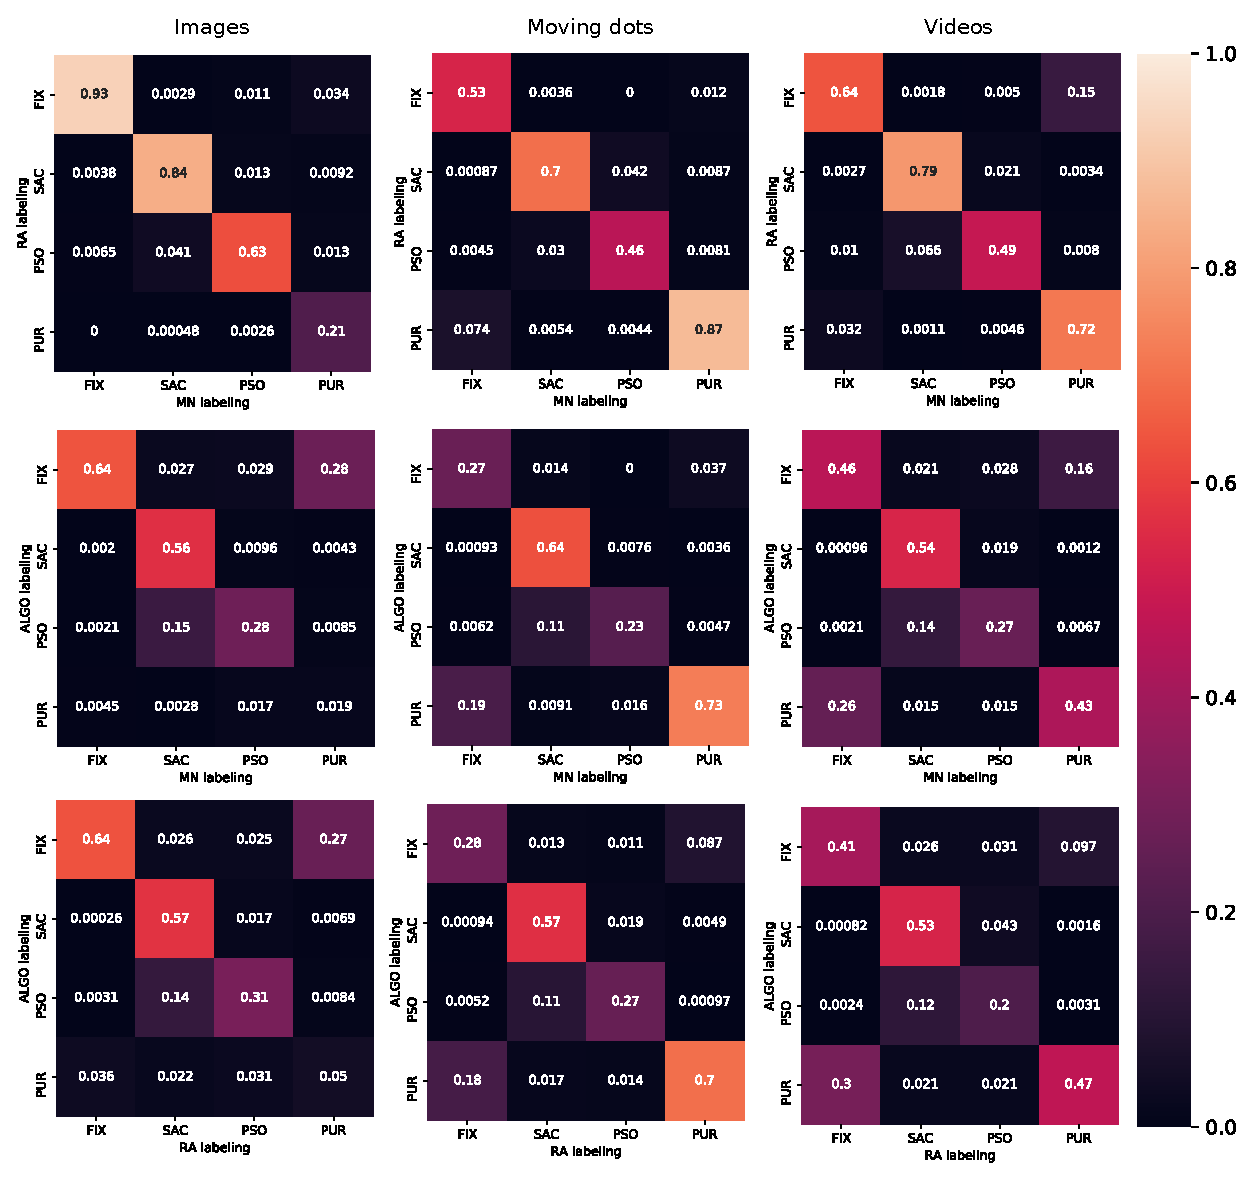
\includegraphics[width=1\textwidth]{img/conf_drawing.eps}
	% figure caption is below the figure
	\caption{Confusion matrices indicating similarity for classification decisions between human coders (top panel), human coder MN and \remodnav (middle panel), and human coder RA and \remodnav (bottom panel) for each of the three stimulus categories. Numbers denote Jaccard index (higher is more similar).}
	\label{fig:conf}       % Give a unique label
\end{figure*}

\begin{figure*}[!ht]
\centering
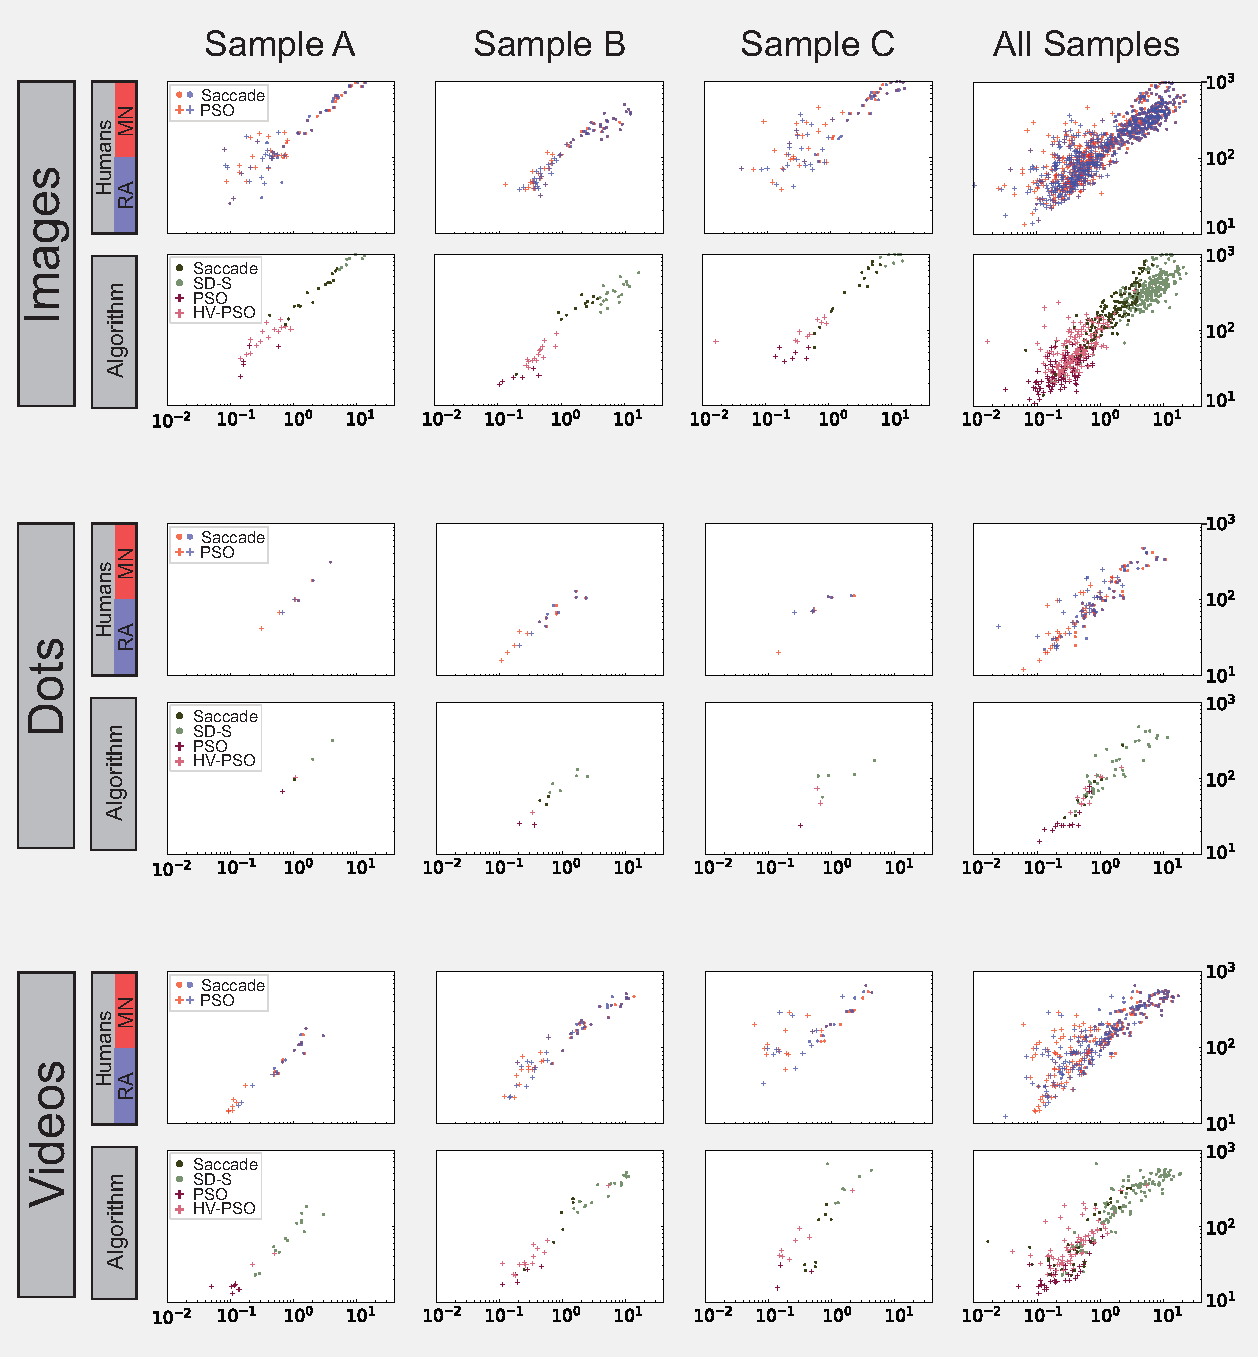
\includegraphics[width=1\textwidth]{Mainseqs_legends.pdf}
\caption{\label{fig:Mainseqs}Overview of use cases to validate to anderson dataset. Three sets of stimuli, namely, images, dots, and videos which are processed by human observers and the algorithm. Sample A shows results that show a good match between the human and algorithmic results,sample B showing acceptable results, while sample C shows a poor match. In the case of the human observers the results of each observer --- represented by either blue or red --- are superimposed onto one another. Event detection done by the algorithm additionally split saccadic events into Segment defining saccades (SD-S) and PSOs to regular and High velocity PSOs (HV-PSO)  }

\end{figure*}
\subsection*{Trial-based data}

\todo[inline]{how do we compare against the "best" LNS algorithm in Andersson2017?}

\todo[inline]{compute RMSD for algo comparison}




%\subsubsection*{Evaluation of events}
\todo[inline]{\textit{Table (or a graphic?) showing duration mean, SD, count and RMSD (tables 3-4, Anderson) for images, dots and videos }}


\subsection*{Prolonged recordings of natural viewing}\label{ana_2}

%discuss inlab vs scanner data
\todo[inline]{\textit{Need to determine exactly which plots and tables will go here}}
%\todo[inline]{\textit{This section contains the analysis of the main sequences -- which I assume is the meat of the thesis. The goal is to have as much information as possible be contained in figures and/or tables (and their captions). We don't pay for those, but we do pay for the main text body.}}
The studyforrest dataset contains eye gaze data from two experimental environments (but the same stimuli); one set taken with the subjects in a MRI machine and the other from subjects in a lab. Of the two, the data taken from the in-lab sessions was far less noisier. After applying the detection procedure to the entire lab data set, a detailed statistical analysis was performed to validate that the characteristics of the detected eye movements fell into biologically plausible ranges. We then applied the algorithm to the scanner data to see how they would compare to the in-lab results \ref{groupcompare}. 

\subsection*{Low-quality data}\label{ana_3}

%
%\onecolumn
%
%%------------------figure------------------------------------------
%\begin{figure}
%\centering
%%\includegraphics[scale=0.35]{figures/MainSeq.png}
%        \caption[Main sequence plot]{Plot of the main sequence, relationship between peak velocity and amplitude of participant ID 24, movie segment 4 (randomly chosen as an example); $r^2$=0.92.}
%        \label{main}
%\end{figure}   
%\begin{table}[h]
%\center
%\begin{tabular}{lcccc}
%\toprule
%\# & duration in $ms$  & amplitude in $^\circ$ & peak velocity in $\frac{^\circ} {s}$ & number of saccades \\
%\midrule
%1	& 	34.99$\pm$0.88 	& 	1.84$\pm$0.15   & 	102.78$\pm$5.43 	& 	884.9$\pm$205.0  	\\
%2 	& 	34.61$\pm$1.11 	&	2.22$\pm$0.16	&  	102.18$\pm$5.99		& 	897.3$\pm$72.1 		\\
%3	&   35.79$\pm$1.19	&   2.26$\pm$0.14 	&  	106.39$\pm$4.72		& 	901.93$\pm$192.9 	\\
%4 	& 	34.81$\pm$1.04 	&  	1.81$\pm$0.10 	& 	74.43$\pm$2.95		&	1148.7$\pm$191.2 	\\
%5 	& 	36.08$\pm$1.19 	&	2.48$\pm$0.17 	& 	97.17$\pm$3.83 		& 	899.0$\pm$240.3 	\\
%6	& 	35.09$\pm$0.78 	& 	1.82$\pm$0.09 	& 	111.79$\pm$3.86 	&	899.1$\pm$151.1 	\\
%7	& 	35.86$\pm$0.63	& 	1.87$\pm$0.10 	&  	89.88$\pm$3.45		& 	959.5$\pm$244.7		\\
%8	& 	34.22$\pm$0.64 	& 	2.55$\pm$0.37 	& 	128.48$\pm$11.09	& 	556.3$\pm$218.8		\\
%
%\bottomrule
%
%\end{tabular}
%\caption {Mean and standard deviations for different metrics grouped by the movie segment.}
%\label{rundetails1} 
%\end{table}
%
%\begin{table}[h]
%
%\centering
%\scalebox{1}{
%\begin{tabular}{lcccc}
%\toprule
%\# & lost signal $\frac{s}{min}$ &$r^2$ & samples removed & slope\\
%
%\midrule
%1 & 4.7		& 	0.889 	&	7.9\%	&	0.510	\\
%2 & 3.8		&   0.856	&	7.0\%	&	0.578	\\
%3 & 5.4 	&   0.847	&	8.9\%	&	0.584	\\
%4 & 4.6 	& 	0.898	&	7.4\%	&	0.573	\\
%5 & 1.2 	& 	0.897	&	2.3\%	&	0.493	\\
%6 & 2.5 	& 	0.880	&	4.6\%	&	0.598	\\
%7 & 0.9 	& 	0.914	&	1.7\%	&	0.516	\\
%8 & 5.3 	&  	0.771	&	8.9\%	&	0.530	\\
%
%
%\bottomrule
%\end{tabular}}
%\caption{Movie segment analysis showing mean values for different metrics over every test subject in a run: Mean value of signal loss in seconds per minute , $r^2$ values for the correlation between peak velocity and amplitude, average percentage of samples removed, average slope of the main sequence. Due to blinks and noise, some samples were removed from the eye gaze data before calculations started. The average percentage of removed samples is illustrated. Across all participants 16\% was the maximum amount of samples neglected and in 93.3\% of the data less than 10\% were disregarded. Included in this removal was the actual pure signal loss during the recording session, meaning samples marked with a null value.}
%\label{rundetails2}
%\end{table}
%
%%------------------figure------------------------------------------
%\begin{figure}[h]
%\centering
%%\includegraphics[scale=0.2]{figures/duration.jpeg}
%        \caption{Histogram of saccade durations. Cut off at 100 $ms$ as for the following bars less than 0.01\% of all data are presented per bin, making it impossible to visualize. Normalized to 1. The largest amount of saccades is very close to minimum duration. The assumed shape of the distribution indicates a gradual decrease to the left, implying the possibility of a number of shorter, yet disregarded saccades. This loss of data can easily be fixed by choosing a less conservative duration threshold. There are many different subjective opinions on minimum saccadic duration, ranging from 10 ms \cite{Duchowski.2007} to 15 ms \cite{Smith.2013}. A more objective approach was provided by Carpenter in 1988 who found a mathematical relation between duration and amplitude of saccades \cite{Carpenter.1988}: $duration=2.2\cdot{}amplitude+21$. According to this equation there are no saccades of less than 21 $ms$. Therefore, a minimum duration of 21 $ms$ was chosen as threshold.}
%\label{dur}
%\end{figure}
%
%%------------------figure------------------------------------------
%\begin{figure}
%\centering
%%\includegraphics[scale=0.2]{figures/amp.jpeg}
%        \caption[Histogram of saccade amplitude]{Histogram of all saccade amplitudes. Cut off at 12 $^\circ$. Normalized to 1. }
%        \label{amp}
%\end{figure}    
%
%%------------------figure------------------------------------------
%\begin{figure}
%\centering
%%\includegraphics[scale=0.2]{figures/pv.jpeg}
%        \caption[Histogram of peak velocity]{Histogram of all saccade peak velocities. Cut off at 400 $\frac{^\circ} {s}$. Normalized to 1. }
%        \label{pv}
%\end{figure}
%
%%------------------table------------------------------------------
%\begin{table}[h]
%
%\centering
%\scalebox{1}{
%\begin{tabular}{lcccccc}
%\toprule 
%    \# & \multicolumn{3}{c}{glissades} & \multicolumn{2}{c}{fixations}\\ 
% & duration in $ms$ & amplitude in $^\circ$ & mean velocity in $\frac{^\circ} {s}$ & duration in $ms$ & number \\ 
%\midrule
%1	& 	39.68 	& 	0.13   	& 	6.60	& 	430.22	&	4965.1  \\
%2 	& 	39.70 	&	0.22	&  	10.93	& 	432.67	&	4865.5 	\\
%3	&   39.77	&   0.19 	&  	7.83	& 	429.49 	&	4975.5	\\
%4 	& 	39.73 	&  	0.09 	& 	5.41	&	394.11 	&	5802.3	\\
%5 	& 	39.73 	&	0.16 	& 	9.87 	& 	445.37 	&	4903.7	\\
%6	& 	39.72 	& 	0.16 	& 	11.65	&	435.96 	&	4823.7	\\
%7	& 	39.72	& 	0.09 	&  	4.92	& 	480.94	&	5403.7	\\
%8	& 	39.81 	& 	0.33 	& 	14.06	& 	469.67	&	3456.3	\\
%
%
%\bottomrule
%\end{tabular}}
%\caption[]{Movie segment analysis for glissades and fixations, showing mean values for different metrics over every test subject per segment, mean value of duration, amplitude, velocity, and number of fixations. Since glissade durations group around the cut off value of 40, it seems that most movements would have been longer than that. This indicates, that the threshold for glissade detection is too low, perceivably because the data used had a higher level of baseline noise than in the experiment by Nyström and Holmqvist.{\cite{Nystrom.2010}} Fixation durations range around a mean value of 420.42 $ms$. Typical values for fixations rarely exceed 400 $ms$. However, the significantly longer fixation durations align with the rest of the eye movements, as saccades were accordingly shorter than typical values suggest. Human gaze in general is preferably directed at the center of the stimulus {\cite{Buswell.1935,Parkhurst.2002}} and the pull towards the center was proven to be strongest in professionally cut Hollywood movie trailers when compared with natural scenes or static images. {\cite{Dorr.2010}} These findings supports the assumption, that participants mainly focused on the center of the screen, which is backed uo by the data. Fixations include small microsaccades, tremor and slow drifts, which allow the viewer to gradually explore the movie stimulus while staying within fixation parameter boundaries.}
%\label{fixgliss}
%\end{table}
%
%%------------------table-----------------------------------------
%\begin{table}[h]
%
%\centering
%\begin{tabular}{lcccccc}
%\toprule
%Movie segment & lab  & scanner & t-statistic & p-value \\
%\midrule
%\rowcolor{lightgray}
%1 	&	0.892 	&	0.740	& 	4.220	& 	0.0039	\\
%
%2	&   0.836 	&   0.841 	& 	0.242	& 	0.8156	\\
%
%3 	&   0.869 	& 	0.793	& 	2.797 	& 	0.0266	\\
%\rowcolor{lightgray}
%4 	&   0.892 	& 	0.590 	& 	7.115 	& 	0.0002	\\
%
%5 	&   0.912 	& 	0.883 	& 	3.789 	& 	0.0068	\\
%
%6 	&   0.917 	& 	0.771 	& 	2.700	& 	0.0306	\\
%
%7 	&   0.921 	& 	0.808 	& 	2.365 	& 	0.0500	\\
%
%8 	&   0.800 	& 	0.821 	& 	0.545	& 	0.6029	\\
%\bottomrule
%
%
%
%\end{tabular}
%\caption[]{Group comparison of lab and scanner data in regard of average $r^2$-value of the main sequence and coefficient of variation per participant. Applying the detection procedure to the rest of data produced similar results. Before computing any t-test comparisons, participants with the IDs 2 and 5 were removed from the scanner data pool. As mentioned in the original study,\footnote{\cite{Hanke.2016}} a large amount of data was lost in their recording session due to signal loss, leaving too little information to detect enough saccades for valid correlation measures. Although there are slight differences in accuracy for the scanner data, the precision level prevails similarly high as for the lab. In direct comparison to the lab data, with a t-test criterion of 0.05, 3 movie segments do not show significant differences in detection accuracy. However, after applying the Bonferroni-Method \footnote{\cite{Abdi.2007}} the detection precision for merely two movie segments is substantially less accurate for scanner data in comparison to lab recordings (highlighted).}
%\label{groupcompare}
%\end{table}
%\twocolumn
%
%\todo[inline]{\textit{For the Comparison of output between Lab and in-scanner data: Need to determine exactly which plots and tables will go here}}
%
%

% no discussion in favor of brief conclusions
%\section*{Discussion}
%
%\subsection*{Comparison to human coders and current algorithms}
%
%
%\subsubsection*{Comparison of outputs from different levels of noise}
\section*{Discussion}\label{dis}
\cite{munn2008fixation} found velocity-based algorithms to perform well in fixation detection during dynamic stimulation.

Remark on the main sequence plots; they look like there are little deviating saccades (which could be PSOs or glissades)

\cite{Komogortsev2013} also successfully employed a combined velocity and dispersion criterion for smooth pursuit identification.

\section*{Conclusion}\label{con} % Optional - only if NO new datasets are included
%This section is required if the paper does not include novel data or analyses.  It allows authors %to briefly summarize the key points from the article. 

Based on the adaptive, velocity-based algorithm for fixation, saccade, and
glissade detection by \cite{Nystrom2010AnData}, we have developed a novel,
robust algorithm for the classification of various eye movements in eye tracking
data from dynamic stimulation. Our algorithm extends the existing software solutions
for eye movement detection in important aspects:
\begin{itemize}
	\item Pursuit classification; add that we're good in that
	\item TODO: What else?
\end{itemize}

Furthermore, our algorithm outperforms previous algorithms in
\todo[inline]{list where exactly we excel and in what way, after results section is finished}
We specifically developed \remodnav to yield robust results with dynamic stimulation,
in particular noisy data such as the eye tracking data recorded simultaneously to fMRI acquisition.
The results confirm that \remodnav is well able to classify eye movements for
movie data, even when the quality of data is low. Therefore, the algorithm is a promising tool for research paradigms with dynamic stimuli where lower data quality is an inherent property of the acquisition procedure, such as simultaneous fMRI and eye gaze recordings, or usage of remote eye trackers.
Furthermore, the algorithm proofed to be well applicable to other types of stimulation. Its classification performance for
as well. \todo[inline]{elaborate on results on Andersons datasets, and include how
the algorithm performs comparable to human coders and contemporary algorithms (or even
exceeds their performance)}.\\
The REMoDNaV algorithm was created with the explicit objective to classify smooth
pursuit eye movements. This is a capability that most contemporary algorithms lack.

As such, REMoDNaV is a versatile tool that provides researchers with a robust
method to classify eye movements obtained from different types of stimulation.
\todo[inline]{note a few advantages that relate to usability of the algorithm:
freely available, platform independent, simple command-line execution, minimum
user input required, adaptivity to the noise level of the data, ..  (i need to
read into how the algorithm is executed again)}


"Data quality is related to accuracy, precision, percentage of data loss, perhaps in addition to a subjective rating from the person responsible for the recording"

"With both dispersion- and velocity-based algorithms, the effect of imprecision can to some extent be alleviated by raising the threshold setting. With a larger dispersion radius, or a higher velocity threshold, sample-to-sample motion can be quicer without enagering the consistency pf fixations. The remedy comes at a price, however. For instance, rasing a velocity threshold above peaks of imprecision will make it so high that some saccades will not be identified."

Problems of current algorithms with low quality data: "Lack of temproal criterion for fixation duration, lack of upper velocity threshold"

Argument pro velocity based criteria (compared to dispersion): Dispersion based algorithms are suspectible to noise and loss of spatiotemporal precision, for velocity based algorithms, filter and thresholds can eradicate implausible accelerations, Nyström \& Holmqvist (book) conclude that velocity algorithms have "good potential for the entire spectrum of [eye tracker] sampling frequencies"



\todo[inline]{from andersson: How does the number of detected events and their
  durations vary with the choice of an algorithm? How similar are the events
  detected by algorithms compared to events manually identified by human
  experts? How similar are algorithms and humans in a simple sample-by-sample
  comparison, which is the most human-like? How similar are our two human
  coders? Are they interchangeable, or will the event detection process depend
  on the human experts we use?  Does the algorithm – human or human – human
  similarity depend on the stimuli used for eliciting the eye movement data,
  i.e. will it differ between static and dynamic stimuli?  What are the
  consequences of trying to detect events in the presence of smooth pursuit
  using improper, i.e. not designed to handle smooth pursuit, algorithms? Is
  this a serious violation, or will such a use provide acceptable
  approximations of the properties of the true (human-identified) events?  How
  congruent are different evaluation techniques, such as similarity based on
  event durations, compared to similarity based on Cohen's Kappa?  Given that
  algorithms do not classify identically with human experts, what types of
  deviating classifications do the algorithms do? Are the deviations random, or
  do they indicate a clear bias in some direction? What area should developers
  focus on improving, to gain the highest marginal improvement (i.e.,
  similarity to humans) of the algorithm?  }


%% we introduce no new data
%\section*{Data availability} % Optional - only if novel data or analyses are included
%Please add details of where any datasets that are mentioned in the paper, and that have not have not previously been formally published, can be found.  If previously published datasets are mentioned, these should be cited in the references, as per usual scholarly conventions.
%\todo[inline]{This will be completed at the end with info on where readers can obtain data and code}


\section*{Software availability}
The latest version of \remodnav can be installed from PyPi via \texttt{pip install remodnav}. It is recommended to use a dedicated virtualenv. The source code of the software can be found on Github \\ (https://github.com/psychoinformatics-de/remodnav). All bugs, concerns and enhancement requests for this software should be submitted via Github. Questions with regard to REMoDNaV can be submitted to NeuroStars.org with a \texttt{remodnav} tag. NeuroStars.org is a platform similar to StackOverflow but dedicated to neuroinformatics. \remodnav is released under MIT license.

%This section will be generated by the Editorial Office before publication. Authors are asked to provide some initial information to assist the Editorial Office, as detailed below.
%\begin{enumerate}
%\item URL link to where the software can be downloaded from or used by a non-coder (AUTHOR TO PROVIDE; optional)
%\item URL link to the author's version control system repository containing the source code (AUTHOR TO PROVIDE; required)
%\item Link to source code as at time of publication ({\textit{F1000Research}} TO GENERATE)
%\item Link to archived source code as at time of publication ({\textit{F1000Research}} TO GENERATE)
%\item Software license (AUTHOR TO PROVIDE; required)
%\end{enumerate}


\subsection*{Author contributions}
%In order to give appropriate credit to each author of an article, the individual
%contributions of each author to the manuscript should be detailed in this section. We
%recommend using author initials and then stating briefly how they contributed.
AD, US, MH conceived and implemented the algorithm.
AD, AW, US, ID, MH validated algorithm performance.
AD, AW, US, ID, MH contributed to the manuscript.

\subsection*{Competing interests}
%All financial, personal, or professional competing interests for any of the authors that
%could be construed to unduly influence the content of the article must be disclosed and
%will be displayed alongside the article.
No competing interests were disclosed.

\subsection*{Grant information}
%Please state who funded the work discussed in this article, whether it is your employer,
%a grant funder etc. Please do not list funding that you have that is not relevant to this
%specific piece of research. For each funder, please state the funder’s name, the grant
%number where applicable, and the individual to whom the grant was assigned.
%If your work was not funded by any grants, please include the line: ‘The author(s)
%declared that no grants were involved in supporting this work.’
Michael Hanke was supported by funds from the German federal state of
Saxony-Anhalt and the European Regional Development Fund (ERDF), 
Project: Center for Behavioral Brain Sciences (CBBS).
Adina Wagner was supported by the German Academic Foundation.

\textit{The funders had no role in study design, data collection and analysis,
decision to publish, or preparation of the manuscript.}

\begin{acknowledgements}
%This section should acknowledge anyone who contributed to the research or the
%article but who does not qualify as an author based on the criteria provided earlier
%(e.g. someone or an organisation that provided writing assistance). Please state how
%they contributed; authors should obtain permission to acknowledge from all those
%mentioned in the Acknowledgements section.
%Please do not list grant funding in this section.
We are grateful to \cite{Andersson2017} for releasing the labeled
eye tracking dataset used for validation under an open-source license.
\end{acknowledgements}

\bibliographystyle{spbasic}      % basic style, author-year citations
\bibliography{EyeGaze,tools}

% \bigskip
% References can be listed in any standard referencing style that uses a numbering system
% (i.e. not Harvard referencing style), and should be consistent between references within
% a given article.

% Reference management systems such as Zotero provide options for exporting bibliographies as Bib\TeX{} files. Bib\TeX{} is a bibliographic tool that is used with \LaTeX{} to help organize the user's references and create a bibliography. This template contains an example of such a file, \texttt{sample.bib}, which can be replaced with your own. Use the \verb|\cite| command  to create in-text citations, like this \cite{Smith:2012qr} and this \cite{Smith:2013jd}.


% See this guide for more information on BibTeX:
% http://libguides.mit.edu/content.php?pid=55482&sid=406343

% For more author guidance please see:
% http://f1000research.com/author-guidelines

% When all authors are happy with the paper, use the 
% ‘Submit to F1000Research' button from the menu above
% to submit directly to the open life science journal F1000Research.

% Please note that this template results in a draft pre-submission PDF document.
% Articles will be professionally typeset when accepted for publication.

% We hope you find the F1000Research Overleaf template useful,
% please let us know if you have any feedback using the help menu above.


\clearpage
\listoftodos

\end{document}
